% translation-source: docs/user/latex/ipr-livre-utilisateur.tex; sha256: 6614ac9dad4001ac98285454b5a382682c781e8b8034fda6aa399ac1d7212716
\documentclass[12pt,a4paper,oneside]{report}
\usepackage[T1]{fontenc}
\usepackage[utf8]{inputenc}
\usepackage[english]{babel}
\usepackage{lmodern}
\usepackage{microtype}
\usepackage{setspace}
\onehalfspacing
\setlength{\parindent}{0 pt}
\setlength{\parskip}{0.5\baselineskip}
\setlength{\emergencystretch}{3em}
% Keep the short instructional paragraphs together, as in the French edition.
\interlinepenalty=10000
\clubpenalty=10000
\widowpenalty=10000
\displaywidowpenalty=10000
\raggedbottom
\usepackage[a4paper,margin=2.4cm]{geometry}
\usepackage{array,longtable,booktabs}
\usepackage{etoolbox}
\newcolumntype{L}[1]{>{\raggedright\arraybackslash}p{#1}}
\AtBeginEnvironment{longtable}{\setlength{\parskip}{0 pt}\interlinepenalty=0}
\usepackage{xcolor}
\usepackage{tikz}
\usepackage{hyperref}
\hypersetup{colorlinks=true,linkcolor=blue!45!black,urlcolor=blue!45!black,
 pdftitle={IPR -- User guide},pdfauthor={IPR project},pageanchor=false}
\newcommand{\touche}[1]{\textsf{#1}}
\newcommand{\chemin}[1]{\texttt{\detokenize{#1}}}
\newcommand{\attention}[1]{\par\noindent\textbf{Remember.} #1\par}
\newcommand{\gestesreglages}{\paragraph{Gestures and keyboard.}
Click the slider to focus it, then use arrow keys to advance by that setting's
declared step. The numeric field accepts direct input confirmed with
\touche{Enter}. Double-clicking the name or slider, or clicking its reset arrow,
restores its reference. Right-clicking the name or slider also exposes reset
and numeric input. Double-clicking the curve graph has a different function.}
\begin{document}
\begin{titlepage}
\centering
\vspace*{2cm}
{\Huge\bfseries IPR\par}
\vspace{0.5cm}
{\LARGE User guide\par}
\vspace{1cm}
{\large Open, develop, compare and export your photos\par}
\vfill
English edition -- alpha prototype\par
Interface integrated into \texttt{dev} (\texttt{b19b4c3})\par
Reconciled reference: 31 October 2026\par
\vfill
\begin{minipage}{0.88\textwidth}
This book describes available commands, their gestures and limitations.
It does not certify rendering for every camera or describe future functions.
Reserved chapters are intentionally empty.
\end{minipage}
\end{titlepage}
\pagenumbering{roman}
\hypersetup{pageanchor=true}
\tableofcontents
\clearpage
\pagenumbering{arabic}
\part{Getting started with IPR}
% translation-source: docs/user/latex/chapters/01-demarrage.tex; sha256: ef75f3d3a176fe7470c6c9d457e2df8fe9be18791e8a567cf18dab62e7f221d6
\chapter{First launch and orientation}
\label{chap:demarrage}
\section{Open a photo}
From the welcome screen, click \emph{Open…} and select an image.
IPR opens its containing folder and displays the folder's images in the bottom
filmstrip. The \emph{File / Open image…} and \emph{Open folder…} menus let you
switch photos or folders. Use \touche{Ctrl + O} for an image and
\touche{Ctrl + Shift + O} for a folder.

A RAW contains data that must be developed; a JPEG, PNG or TIFF already contains
a rendered image. A DNG can contain different kinds of data: its extension alone
does not establish that it contains a RAW mosaic. Use the dialog filters to see
which files the installed build offers.

\section{The four working areas}
\begin{center}
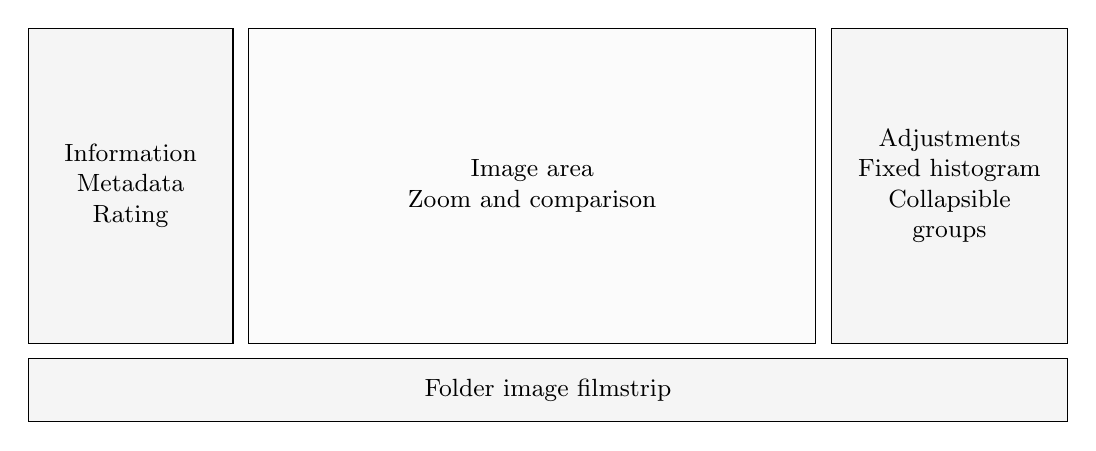
\begin{tikzpicture}[x=1cm,y=1cm,every node/.style={font=\small,align=center}]
\draw[fill=gray!8] (0,1) rectangle (2.6,5);
\draw[fill=gray!3] (2.8,1) rectangle (10,5);
\draw[fill=gray!8] (10.2,1) rectangle (13.2,5);
\draw[fill=gray!8] (0,0) rectangle (13.2,0.8);
\node at (1.3,3) {Information\\Metadata\\Rating};
\node at (6.4,3) {Image area\\Zoom and comparison};
\node at (11.7,3) {Adjustments\\Fixed histogram\\Collapsible\\groups};
\node at (6.6,0.4) {Folder image filmstrip};
\end{tikzpicture}
\end{center}
This diagram shows the interface layout; it is not a screenshot.
The \emph{View} menu can hide Information, Histogram or Filmstrip.
Click a group header to expand or collapse its settings. Collapsing does not
reset the values.

\section{A simple first development}
\begin{enumerate}
\item Open a photo and wait for processing to finish.
\item Check its profile, then adjust exposure under \emph{Light}.
\item Compare the original and current states; zoom in to check details.
\item Adjust color, then noise and sharpening if needed.
\item Export a copy using the summary described in Chapter~\ref{chap:export}.
\end{enumerate}

\section{Understand ongoing processing}
A badge appears over the image when processing takes sufficiently long.
A camera preview may appear before IPR's development; it is explicitly identified.
The RAW / Profile description stays stable during an ordinary adjustment render
so controls do not move. The message at the bottom of the window provides details
and errors.

\attention{The badge is generic, not a percentage progress bar. It does not yet
expose every engine stage separately. The absence of a badge does not replace
checking a possible error message.}

\section{Edits and saving}
Settings are stored in an \chemin{.ipr} sidecar beside the source, for example
\chemin{photo.CR3.ipr}. These edits do not rewrite the source file. Keep the
sidecar with the image when moving or backing it up; check folder write access.
Storage is automatic and delayed: wait for processing and check any save
warnings before quitting.

\emph{Save adjustments} and \touche{Ctrl + S} immediately write the ready
image's sidecar. Read the success or failure message; automatic saving also
remains active. \touche{Ctrl + Q} quits outside a modal dialog.

\attention{A sidecar is neither a copy of the photo nor an export. Interface
preferences are stored separately in an INI file.}

% translation-source: docs/user/latex/chapters/02-navigation-comparaison.tex; sha256: 1f9404cd44ced347dbc88730edc212d7639d19454714d8714ef40131b766c876
\chapter{Navigation, zoom and comparison}
\label{chap:navigation}
\section{Move between images}
Click a thumbnail to open its photo. Its outline and bold name identify the
image actually open, independently of multiple-selection checkboxes. When the
filmstrip is collapsed, previous and next buttons appear at the bottom right
of the image area. Hovering shows the destination name; navigation stops at
the folder boundaries.

The centered button above the filmstrip collapses it. When hidden, this button
returns to the bottom of the view and reopens it. Its state is remembered.
Arrow keys are not global shortcuts for changing photos.

\section{Examine details}
Click the photo to switch from fit-to-view to a magnified view, then click
again without moving the mouse to return to fit-to-view. When the image
extends beyond the view, hold the left mouse button and drag to inspect it.
Clicking an empty margin does not trigger zoom.

\paragraph{Keyboard and wheel.}
\touche{Ctrl + +} zooms in; \touche{Ctrl + $-$} zooms out.
\touche{Ctrl + 0} fits the view and \touche{Ctrl + 1} displays at 100\,\%.
\touche{Ctrl + wheel} zooms around the pointer. Without Ctrl, the wheel pans
the magnified image; \touche{Shift + vertical wheel} pans horizontally.
The corresponding buttons remain available above the photo.

\attention{100\,\% means one preview pixel per view unit; the interactive
preview may be smaller than the full-resolution source. Export is rebuilt
independently at its intended resolution.}

\section{Show a split comparison}
Click \emph{Before/after} or use \touche{Ctrl + Shift + Y} when both previews
are ready. The original is on the left and the current state on the right.
Drag the divider to set their widths. Both sides share zoom and pan.

\section{Temporarily view the original}
Focus the image view, then hold \touche{Space}. Releasing returns to the
previous presentation, including split comparison if active. The \emph{Original}
button has the same effect while held down. This does not apply to typing in
a numeric field. Changing photos resets the view and comparison.

\attention{The original is the development reference exposed by IPR, not the
raw sensor mosaic or necessarily the camera JPEG. Changing the development
profile may change this reference.}

\section{Photo context menu}
Right-click the view to open photo actions: export, adjustment reset and file
commands. Right-clicking does not zoom. With the view focused,
\touche{Shift + F10} or the Menu key also opens this menu.
Reset requires confirmation; there is no general undo.
Save is connected; Duplicate remains disabled until its engine connection
is available in this reference version.

% translation-source: docs/user/latex/chapters/03-informations-selection.tex; sha256: d6262e09b4a7770461e960518bb3c510f2e2d54c066a2e8584fc3ce8f21c3dd8
\chapter{Information, rating and selection}
\section{Read image information}
The left panel describes the open photo: name, available date, storage,
dimensions, camera and other known metadata. Missing information must not be
interpreted as a measured zero. Available shooting information below the
histogram helps you read ISO, focal length and exposure time.

\section{Rate and flag a photo}
Click one of the five stars to assign a rating from 1 to 5. Clicking the selected
rating again resets it to zero. Click to toggle the flag. Choose a red,
yellow, green, blue or purple label; clicking the same color removes it.
These organizational choices do not recolor pixels and are not mixer bands.

No numeric rating or flag shortcut is currently declared. Use the Information
panel controls.

\section{History and snapshots}
Under the labels, the left panel lists the steps of the open photo, the most
recent at the top. A drag of a slider or wheel, a moved curve point, a typed
value or a profile choice each count as one step. The last hundred steps are
saved in the photo's sidecar and come back when it is reopened.

\emph{Undo} and \emph{Redo} are in this section and in the \emph{Edit} menu.
Clicking a step returns to it; more recent steps appear dimmed and stay
available until the next edit. Undoing a profile change develops the photo
again.

To remove an edit from the middle of the history, right-click its step and
choose \emph{Delete this step}, or press \touche{Delete} when the list has the
focus: the current step is then removed. Later steps are replayed without this
edit and keep what they changed themselves. The opening step cannot be removed.

A snapshot keeps the current state under a name. Type the name, then choose
\emph{Create}; clicking the snapshot restores it as a new step.

\attention{Once saved by this version, a sidecar can no longer be read by an
older version of IPR. A sidecar written by a more recent version opens as
read-only.}

\section{Copy and paste settings}
On a ready image, choose \emph{Edit > Copy settings} or
\touche{Ctrl + Shift + C}. Open the destination photo, wait for processing,
then choose \emph{Paste settings} or \touche{Ctrl + Shift + V}.
These commands are also available by right-clicking the open image.
The copy is a snapshot: subsequent source edits do not alter it. It remains
available during the session, even after switching folders.

Pasting replaces all edits, including curves, mixer and grading. It preserves
the destination profile, calibration, optics, automatic white balance and
rating. If the source uses as-shot white balance, the destination uses its
own as-shot balance; custom temperature and tint are copied as absolute
values. Two cameras will not necessarily produce the same color.
There is no selection of individual groups to paste yet; a paste can be undone
like any other history step.
\touche{Ctrl + C} and \touche{Ctrl + V} remain available in text fields.

\section{Copy edits to multiple photos}
\begin{enumerate}
\item Open the photo whose settings you want to copy.
\item Check destination thumbnails or use \touche{Ctrl + click}; do not
confuse a checked box with the open image. The counter shows selected files.
\item Right-click and choose \emph{Apply the open image's settings to the selection},
also in the \emph{Edit} menu. Check the result message.
\item Uncheck files or use the clear-selection button.
\end{enumerate}
This writes edits into destination sidecars. It is not limited to the currently
expanded group. Destination RAW profiles and automatic white balance are not
blindly copied between cameras; destination organizational metadata is preserved.

\attention{This is batch application of edits, not the multiple-export
command. \touche{Ctrl + click} only toggles the targeted thumbnail without
opening it; an ordinary click opens it without clearing the selection.
Shift-click range selection is not implemented.}

\section{Filmstrip badges}
The open thumbnail's badge may show rating, flag and label. No badge on another
thumbnail does not mean that it has no rating or edits: those data are not yet
exposed for every model row.

\section{Right-click a thumbnail}
The menu targets the thumbnail under the pointer. For a photo other than the
open one, first choose \emph{Open this image}: right-clicking alone neither
loads it nor changes multiple selection. Editing actions remain disabled
until that target is open, avoiding an accidental reset or export of the
previous photo.

\emph{Duplicate file and settings}, associated with the reserved
\touche{Ctrl + D} shortcut, is intended to make a physical copy and a consistent
sidecar, not a developed TIFF or virtual copy. This command still awaits its
engine interface and is disabled in the version described.

\part{Integrated adjustment families}
% translation-source: docs/user/latex/chapters/04-raw-profils.tex; sha256: a0c0905dd992d79083ed2f7d606aa1c18b4a5e64831463414261424d5e8d6b39
\chapter{RAW development and profiles}
\section{Choose the starting rendition}
The \emph{RAW Development / Profile} group selects a DCP profile compatible
with the photo. Choices depend on the camera, installed profiles and build.
Check the description of the profile actually used, not just the requested
name in a list.

A camera profile defines a starting rendition: it may change colors, contrast
and apparent brightness before edits. Two applications need not produce
identical pixels from similarly named profiles. This group does not treat
a JPEG as a RAW and apply a camera DCP to it.

\section{Change profiles}
Select a list entry, wait for processing, then compare. The engine can avoid
a complete re-decode when a compatible buffer is available; the interface
indicates this capability. It does not guarantee that every development
change is instantaneous. Commands that could change development are disabled
during some operations.

\section{Automatic white balance and calibration}
The \emph{Automatic white balance} checkbox appears here once. Manual
temperature and tint remain under \emph{Color}. Do not confuse automatic
balance, shooting temperature and the DCP profile.

RAW calibration is an advanced preference, accessed using
\touche{Ctrl + comma}, \emph{Advanced · RAW} tab. Compatible cameras and modes
have default calibration. Check its applied status in the description:
an enabled checkbox does not guarantee that an unknown file has an available
characterization.

\attention{The advanced choice concerns the open image and its sidecar, not
a new global preference for every subsequent photo. Change the calibration
manifest only under a controlled protocol.}

\paragraph{Example.}
To compare profiles, keep edits identical, disable corrections unnecessary
for the test, change only the profile, then inspect skin tones, vivid colors
and highlights. Record white balance for reproducibility.

% translation-source: docs/user/latex/chapters/05-lumiere.tex; sha256: 20046c985a406213c2f06ec61857c03dcac1c7cd28fcd7f27adae0d8386db34a
\chapter{Light and histogram}
\section{Read the fixed histogram}
The histogram stays at the top of Adjustments while scrolling. It describes
the processed current sRGB preview, not raw sensor values. End indicators
flag preview values at their limits; they do not directly measure sensor
saturation.

Reading zones are Blacks(0--10\,\%), Shadows(10--33\,\%),
Exposure(33--66\,\%), Highlights(66--90\,\%) and Whites(90--100\,\%).
These are visual references, not hard slider influence boundaries.

\section{Controls}
\begin{longtable}{@{}L{3cm}L{2.8cm}L{7.8cm}@{}}
\toprule Setting & Range & Usage\\\midrule\endhead
Exposure & $-5$ to $+5$ EV & Adjust overall brightness; begin with small changes.\\
Contrast & $-100$ to $+100$ & Strengthen or soften tonal separation.\\
Shadows & $-100$ to $+100$ & Brighten or darken dark regions, not just the black endpoint.\\
Blacks & $-100$ to $+100$ & Adjust the darkest tones and the image's tonal foundation.\\
Highlights & $-100$ to $+100$ & Moderate or strengthen bright tones.\\
Whites & $-100$ to $+100$ & Adjust tones nearest white.\\
\bottomrule
\end{longtable}
Zero is the reference for all six controls. On a RAW with camera signal and
DCP, exposure operates before the profile: $+1$EV doubles the linear signal
there, not necessarily TIFF values after the curve. Without that camera
context, the gain is applied to the linear master. The \emph{Grayscale}
checkbox in this group toggles monochrome rendering.

\section{Suggested procedure}
Set exposure first, then shadows and highlights, followed by blacks, whites
and contrast. Revisit earlier steps as needed: these controls interact
visually. Raising shadows also reveals existing noise. A highlight adjustment
cannot recreate information absent from the source.

\paragraph{Example.}
For backlighting, try slightly lowering highlights and moderately raising
shadows rather than immediately pushing both sliders to their extremes.
Hold \touche{Space} in the image view to compare, then inspect transitions
using \touche{Ctrl + 1}.
\gestesreglages

% translation-source: docs/user/latex/chapters/06-courbes.tex; sha256: c9120e88bac82ef65f76b3799e02874eb224ebbb0f5c048893e981b5bf2a188e
\chapter{Tone curve}
\section{Choose a channel}
Select luminance or the red, green or blue channel using the module buttons.
The diagonal represents the reference mapping. Editing a channel can introduce
a color cast even if its curve resembles the luminance curve.

\section{Manipulate points}
Double-click the graph to add a handle, drag it to change the curve, and
right-click an interior handle to remove it. Endpoints do not behave like
interior points. Avoid accumulating closely spaced points: a simpler curve
is easier to control.

Use reset for the current curve or all curves as appropriate. Double-clicking
this graph \emph{adds a point}: it is not the sliders' reset gesture.
No dedicated keyboard shortcut for adding/removing points is declared.

\section{Monochrome background}
The gray silhouette shows the current preview's luminance and stays monochrome
when an RGB curve is selected. It is a post-render reference, not the exact
histogram of the linear signal entering the curves.

\paragraph{Example.}
For gentle contrast, start with two widely spaced interior points, lower
the dark region slightly and raise the bright region slightly. Compare using
\touche{Ctrl + Shift + Y}; watch transitions rather than seeking a perfect
geometric shape.

% translation-source: docs/user/latex/chapters/07-couleur.tex; sha256: 26daf42a5ca80611cc543e8d13bc3576ca31df4a090b8ca9af27366d4c953719
\chapter{Global color}
\section{Temperature and tint}
Temperature spans 2\,000 to 50\,000 K; tint spans $-150$ to  $+150$.
Temperature shifts warm/cool balance; tint corrects the green/magenta axis.
Slider bands are indications, not a contractual swatch of the result.
Automatic white balance is in the RAW group.

The reference temperature depends on photo development; it is not always
5\,200 K or6\,500 K. Reset returns to that reference, not zero kelvin.
Tint resets to zero in the current interface. Units or values shown by
another application do not guarantee exact numeric correspondence.

\section{Vibrance and saturation}
Both controls span$-100$ to  $+100$, with zero as reference. Saturation changes
overall color richness. Vibrance seeks a more selective effect based on
colors already present; it is not simply weaker saturation. Strong effects
on vivid colors may also change their apparent brightness.

\paragraph{Example.}
Begin with a small temperature correction, then adjust tint. Add moderate
vibrance for dull colors and inspect skin tones, reds and yellows.
Adjust global saturation while viewing both the whole image and already
colorful regions. Hold \touche{Space} in the view to compare with the original.

\attention{Color validations depend on the starting rendition, profile and
camera. Extreme values are useful tests, not a promise to reproduce Lightroom
exactly.}
\gestesreglages

% translation-source: docs/user/latex/chapters/08-melangeur.tex; sha256: 73c6252c6105f9fddd2f61610821a5a019c6de748efd8f530aa1fd1402108b9f
\chapter{Color mixer}
\section{Select a color family}
The eight circles select reds, oranges, yellows, greens, cyans, blues, purples
or magentas. Purple and magenta are distinct bands. The colored name confirms
the active band. Changing circles changes the displayed controls without
clearing other bands' settings.

\section{Hue, saturation and luminance}
Each band has three $-100$ to  $+100$ controls with zero as reference. Hue shifts
the family toward its neighbors, saturation changes color richness and
luminance changes brightness. Families overlap gradually: a boundary color
may respond to several bands. This is not object selection.

\paragraph{Example.}
For an orange flower, select oranges first, try a small luminance change,
then saturation, and inspect neighboring reds and yellows. If the starting
rendition is already too red, check profile and white balance before routinely
compensating for it with the mixer.

Compare using \touche{Ctrl + Shift + Y}. No shortcut for selecting the eight
circles is declared; use the circles or focus navigation.
\gestesreglages

% translation-source: docs/user/latex/chapters/09-grading.tex; sha256: 9d1d80ab978ab206b1b2a0df2674872b7f4b71a1c8c6de39f41a0e42038bbe46
\chapter{Color grading}
\section{Choose a tonal region}
The buttons select shadows, midtones, highlights or the \emph{Global} wheel.
Each region retains its own settings independently. Unlike the mixer,
selection concerns a tonal region, not objects already having a particular color.

\section{Use the wheel}
Click the wheel and drag the selection. Angle selects hue; distance from
the center controls intensity. While dragging beyond the edge, interaction
continues at maximum intensity; there is no need to pick up the handle
again on each turn. The 0 to 100 \emph{Intensity} control also supports numeric
input. At zero, the region's color effect is neutral even if its hue is retained.

\section{Luminance, blending and balance}
Region luminance spans $-100$ to  $+100$. Blending, from 0 to 100, changes tonal
region overlap; balance, from$-100$ to  $+100$, shifts their balance.
The Global wheel applies an overall correction instead of selecting only
shadows, midtones or highlights.

\paragraph{Example.}
Give shadows a weak bluish tint and highlights a weak warm tint. Check
midtones and skin tones, then compare by holding \touche{Space} in the view.
Avoid pushing all three regions to maximum when assessing a natural rendition.

\paragraph{Keyboard.}
The intensity slider supports arrow keys, numeric input and double-click
reset as described for adjustments. Angular wheel control with arrow keys
is not currently declared.

% translation-source: docs/user/latex/chapters/10-effets.tex; sha256: 631ea3a63b0b3d80150e1fbea4a21e8e3cbb4900e4f11c5a37a7ef55d7ce884c
\chapter{Effects}
\section{Choose an effect}
\begin{longtable}{@{}L{3.6cm}L{2.8cm}L{7.2cm}@{}}
\toprule Control & Range & Intention\\\midrule\endhead
Texture & $-100$ to $+100$ & Soften or enhance small details.\\
Clarity & $-100$ to $+100$ & Change structural presence and local contrast.\\
Dehaze & $-100$ to $+100$ & Change apparent haze and tonal separation.\\
Grain & 0 to 100 & Add grain; this is not noise reduction.\\
Gaussian blur & 0 to 20 & Soften globally; not a complete depth-of-field simulation.\\
\bottomrule
\end{longtable}
All these controls have zero as reference. Negative texture or clarity is
not equivalent to the dedicated noise-reduction module.

\section{Check artifacts}
Inspect edges, sky transitions and fine textures after a strong correction.
Increased clarity can make noise more visible; excessive smoothing can make
surfaces look artificial. Also check delivery size: detail that looks pleasant
at high magnification may be excessive in fit-to-view.

\paragraph{Example.}
On a hazy landscape, start with a small dehaze correction, then rebalance
light if needed. Compare using \touche{Ctrl + Shift + Y} and inspect sky/building
boundaries at \touche{Ctrl + 1}.
\gestesreglages

% translation-source: docs/user/latex/chapters/11-bruit.tex; sha256: e174c4361e3f9d35ac2f47cd6819d91abd76e188c2fea467f445ef9deb83be27
\chapter{Noise reduction}
\section{Master control and advanced settings}
The \emph{Noise reduction} slider spans 0 to 100, with zero as reference.
It controls luminance and color together, with a different progression for
each component. Its scale is not equivalent to Lightroom's. Open
\emph{Advanced} to adjust the two components independently. A custom pair
may display \emph{Custom} on the master control.

\section{Separate two components}
\emph{Luminance noise} targets brightness fluctuations; \emph{Color noise}
targets unwanted chromatic variations. Both controls span0 to 100 and default
to zero. Their presence does not mean the engine uses AI equivalent to another
application's.

\section{Experimental RAW path}
\emph{Signed RAW signal, before profiles (experimental)} is off by default.
For a compatible RAW and camera context, it selects denoising before optical
corrections and DCP rendering. Changing this may require re-decoding.
Without a compatible context, the classic path remains active; the checkbox
alone therefore does not establish the effective processing path.
This is session state, not an option guaranteed to persist in the sidecar.
Do not confuse strengths with this path selection. The current prototype
is not neural. Stabilization does not mean it perfectly preserves all details;
the neural approach is planned for beta and is not available in this version.

\section{How to use it}
First correct the useful exposure and examine a fairly uniform dark region,
then a textured region. Gradually increase color reduction if colored blotches
are visible. Then adjust luminance while checking hair, fabric and fine detail.
Return to fit-to-view to assess the overall impression.

\paragraph{Example.}
For a high-ISO photo, do not judge only the dark background. Also compare
texture and a sharp edge. Use \touche{Ctrl + 1}, remembering the preview's
resolution, then inspect a full-resolution export before a final detail decision.

\attention{Stronger noise reduction may remove real detail. A Lightroom
reference made with AI denoising is not an equal-algorithm comparison.}
\gestesreglages

% translation-source: docs/user/latex/chapters/12-nettete.tex; sha256: 4089066b3eb0e45781a918a83160335b8cd25bd7d327ec73434782d92cdf6150
\chapter{Sharpening}
\section{The three controls}
\emph{Sharpening amount} spans 0 to 200 and controls enhancement strength.
\emph{Sharpening radius} spans 0.3 to 3.0 and sets its scale, with 1.0 as reference.
\emph{Sharpening masking} spans 0 to 100 and controls selectivity.
Amount and masking have zero as reference.

\section{Procedure}
Assess noise first, then increase sharpening amount slightly. Vary radius
carefully and watch high-contrast edges. Seek improved readability without
visible fringes or amplification of uniform areas. Enhancement cannot recover
focus information that is genuinely absent.

\paragraph{Example.}
On a portrait, inspect the eye edge and skin texture, not just hair.
Switch between \touche{Ctrl + 1} and \touche{Ctrl + 0}. Hold \touche{Space}
to compare with the reference; then inspect an export at delivery size.
\gestesreglages

% translation-source: docs/user/latex/chapters/13-optique.tex; sha256: 84aac22621b44c67d2987f3626ac197ff72abbc0a7f619306cc4845b444eaf15
\chapter{Optical corrections}
\section{Enable available corrections}
\emph{Optical corrections} is near the end of the list, before Export.
Its checkboxes control lens correction and chromatic aberration reduction.
Capabilities depend on the RAW, metadata and available lens profile.
Read diagnostics to see corrections actually applied and whether an LCP
profile is missing.

A camera DCP and lens LCP have different roles. An enabled checkbox is not
proof that every geometric, vignetting or chromatic correction could actually
be calculated.

\section{Compare correctly}
Inspect straight lines near image edges, corner brightness and fringes along
high-contrast edges. Vignetting correction may brighten borders and change
the overall impression of brightness. For color-development comparisons,
keep optical settings identical or disable them consistently on both sides.

\paragraph{Keyboard.}
Use \touche{Tab} to focus a checkbox and \touche{Space} to toggle it.
Space displays the temporary original only in the image view. There is no
global optical-correction shortcut.

\part{Customize and deliver}
% translation-source: docs/user/latex/chapters/14-preferences.tex; sha256: 3f3bf1410806eecfe6057b8598cd3c1d21193c3dbe336d576d0170b216f54920
\chapter{Preferences and layout}
\section{Open preferences}
Use \emph{Preferences} or \touche{Ctrl + comma}. The three tabs are
\emph{Interface}, \emph{Appearance} and \emph{Advanced · RAW}.
Interface preferences are distinct from each photo's edits.

\section{Interface}
Show or hide Information, Histogram and Filmstrip; choose Adjustments width
(260--360 px) and information text size(10--20 px). The same panels can be
hidden from the View menu.

Handles between side panels and the image view resize Information(210--300 px)
and Adjustments. The handle above the filmstrip sets its height(100--260 px).
Drag, or focus a handle and use arrow keys in 10 px increments.
Double-click restores the usual size. Dimensions are stored in the INI file.

\section{Appearance}
Available palettes are Burgundy, Off-white, Matte black, Navy blue and Current
gray. They apply to panels and preferences. The photo background is independent:
changing palettes does not replace that choice. Navy blue and burgundy
backgrounds use gradients.

\attention{For fine color assessment, a neutral gray background limits the
influence of colored surroundings. The interface palette does not change
exported pixels and is not an ICC display profile.}

\section{Advanced · RAW}
This tab exposes calibration for the open image, its manifest and profile/
calibration reset. This last button differs from \emph{Reset adjustments},
which restores edit references but does not automatically erase every RAW
development choice. General reset is also available with
\touche{Ctrl + Shift + R} and requires confirmation for the open photo.

\section{Persistence and adjustment state}
Expanded sections, dimensions, colors and some interface choices are remembered.
The INI path appears in preferences. For manual editing, close IPR and keep
a backup of the file.

A bold numeric-control name and a dot on its section indicate a difference
from its reset value. This does not yet cover all curves, checkboxes and
recipes; it is not a comprehensive saved/unsaved indicator.
Extended-hover explanatory tooltips remain planned for beta.

% translation-source: docs/user/latex/chapters/15-export.tex; sha256: 998176f47aaec2bc3beb8d847db896979f9cff794a16e3b1b814f220eba394e1
\chapter{Export an image}
\label{chap:export}
\section{Choose a format}
Open Export and select a format. JPEG Quality appears only for JPEG;
it spans 1 to 100, with 92 as reference.
\begin{longtable}{@{}L{2cm}L{4.6cm}L{7cm}@{}}
\toprule Format & Current encoding & Use and limits\\\midrule\endhead
JPEG & sRGB,8 bit & Everyday copy; lossy compression, adjustable quality.\\
PNG & sRGB,16 bit & High-bit-depth rendered image; no JPEG Quality control.\\
TIFF & sRGB,16 bit & Comparison reference or high-bit-depth rendered exchange.\\
DNG & Linear RGB,16 bit, sRGB primaries & Contains developed rendering, not the original RAW mosaic.\\
\bottomrule
\end{longtable}
These describe the current exporter, not every theoretical format capability.
This panel offers no user-selectable output gamut or resizing control.

\section{Destination and confirmation}
\begin{enumerate}
\item Wait for development, then click \emph{Choose destination…}.
\item Check name, folder and type in the native dialog. The panel's format
is initially selected; changing type also changes the requested format.
\item In \emph{Review export}, check format, encoding, full-resolution
dimensions and requested destination.
\item Click \emph{Export}, or \emph{Cancel} to return without writing.
\item Read the final message for the actual published file or error.
\end{enumerate}
\section{Export a selection}
\emph{Export selection} processes selected images using their respective
recipes at full resolution, one after another. Names are made unique without
replacing existing files. Watch progress and named failures; cancellation
between images does not imply immediate interruption of native development
already running.
The extension follows the format. If a name exists, the exporter adds an
available number instead of overwriting. The final path may therefore differ
from the requested name in the summary.

\attention{The summary does not reserve the final name. Another process may
create a file between selection and writing; the exporter still protects
against collisions.}

\section{Gestures and controls}
\touche{Tab} navigates dialog controls and \touche{Enter} confirms active input.
Explicitly use Export to start writing. \touche{Ctrl + E}, the File menu and
the photo's right-click menu open the same destination and summary workflow.
Do not confuse export with automatic sidecar saving.

For reproducible testing, export a neutral reference and an edited state
with identical profile, white balance, optical corrections and format.
Record settings: an IPR TIFF alone is not a complete, reliable recipe record.

% translation-source: docs/user/latex/chapters/16-depannage.tex; sha256: cbf3419c9b5a3f8fab807eacd480befd6b0240f42f1f53c0d66a95c7a6dc7021
\chapter{Checks and troubleshooting}
\section{A command seems unavailable}
Check that a photo is open, wait for processing and confirm it is a RAW for
camera-development commands. A missing profile is not necessarily a list error:
availability depends on installed files and compatibility.

\section{The photo differs from another application}
Compare the same file, framing and neutral state first. Check camera profile,
white balance, calibration, optical corrections, noise and sharpening.
An identical displayed temperature does not alone establish equal development.
The viewing background and color-management path may also affect comparison.

\section{Settings reappear on opening}
Look for the \chemin{.ipr} sidecar kept with the photo. Restoration is intentional.
Use the reset appropriate to your goal instead of immediately deleting files.
Keep a backup before manually changing a sidecar or configuration.

\section{Saving or export fails}
Read the bottom status message. Check free disk space, folder permissions,
availability and file locks. A sidecar failure is not a successful export.
The export success message gives the actual path, including any added number.

\section{A function is not described}
Crop, masks and AI panels are reserved in this edition. Complete filmstrip
badges, comprehensive modified-group indicators and detailed engine states
remain future work, not hidden commands. User visual validation and testing
other cameras remain necessary despite automated interface tests.

\part{Geometry}
% translation-source: docs/user/latex/chapters/17-recadrage-geometrie.tex; sha256: 4da6db7b88fb9552aeb74476f21d57b193c80420d0c1b78ea4b2895c0a201473
\chapter{Cropping and geometric effects}
% Reserved family, as in the technical manual. No content until work starts.

\part{Assemble}
% translation-source: docs/user/latex/chapters/22-assembler.tex; sha256: b74ee6fa2877dd8f8dcd907849cbcae38b55ff53588a797353fc5bd1438bdafe
\chapter{Assembling several photos}
The \emph{Assemble} tab, at the top of the right panel, makes a new image from the
photos ticked in the ribbon. The original photos do not change. The work runs in the
background and can be cancelled; you can keep browsing your images meanwhile.

\section{Stacking to reduce noise}
Stacking averages several views of the same scene, at the same exposure. Noise falls
with the square root of the number of views: four views halve it, sixteen divide it by
four. Details remain, because they are the same from one view to the next.

\begin{enumerate}
\item Tick at least two photos in the ribbon.
\item Choose the \emph{Reference}: the final image keeps its framing. The middle photo
is proposed, as it stays the closest to the others.
\item Click \emph{Assemble}.
\item Look at the preview, choose the format, then \emph{Export}.
\item \emph{Open the result} brings it into the editor, for further editing.
\end{enumerate}

The views are registered automatically: a tripod is not needed. The result is cropped to
the area common to all views. What moves from one view to the next, like a passer-by, is
left out if it appears in only a minority of views. A view that cannot be registered or
whose exposure differs too much is left out, and the message says so.

\section{Choosing the format}
\begin{itemize}
\item \emph{DNG}: the camera's signal, already corrected for the lens, with no profile
applied. The file reopens like a RAW: profile, balance and settings stay free.
\item \emph{TIFF}: the image rendered in 16 bits with the reference's profile, readable
everywhere.
\end{itemize}
An existing file is never replaced: the name receives a number.

\section{Assembling a panorama}
Choose \emph{Panorama} at the top of the tab. Photos taken from the same place make one wide
view, on one row, horizontal or vertical, or on several rows. Tick them in the ribbon, in any
order, then click \emph{Assemble}.

Let neighbouring photos overlap by a quarter to a third, and keep the same shooting settings.
A photo that overlaps no other, or taken at another focal length, is left out, and the message
says so.

\begin{itemize}
\item \emph{The bottom of the view} is what the panorama leans on: it stays level, and the
crop rather takes from the top.
\item \emph{Projection}: \emph{Automatic} chooses from the field covered. \emph{Flat} keeps
lines straight over a narrow field, \emph{Cylindrical} suits a long sweep, \emph{Spherical} a
field wide in both directions.
\item \emph{Edges}: a panorama seldom has straight edges. \emph{Crop} keeps the largest
rectangle of real pixels; it is the default, and nothing is invented. \emph{Fill} keeps the
whole surface and completes the corners with pixels invented from the rest of the image.
\emph{Leave empty} keeps the empty corners, to crop later in the Geometry tab.
\end{itemize}
Filling is convincing on a sky. On rock or vegetation, look at the result at 100~\%: some blocks
may be out of place. The final message tells the share of invented pixels.

Hand-held, a close foreground moves from one photo to the next: the seams run where it shows
least as far as they can, but turn around the camera rather than around yourself.

\section{Photographing the Moon}
A small subject on an empty background, like the Moon, gets one more treatment. The
deformations of the atmosphere are corrected on the subject, and only the sharpest half
of the views is merged there. The rest of the sky keeps all the views. The message tells
when this correction took place. In our measurements at 200~mm, the choice of the sharp
views brings most of the gain: the longer the series, the more good views to choose from.

\section{Limits}
\begin{itemize}
\item The capture settings must stay the same: stacking is not HDR.
\item A near object shot hand-held may keep a slightly soft edge: it does not move like
the background.
\item The work needs about 400~MB of temporary disk per 32~Mpx photo for a stack, and twice
that for a panorama.
\item A panorama does not warp its edges to fill the frame.
\item A colour profile for the camera is required.
\end{itemize}

\part{Reserved families}
% translation-source: docs/user/latex/chapters/18-masques-retouche.tex; sha256: df922ca18b03a116c0eeb8f78f6170e72f0fc7864359dd88335cf82c0fc6bfab
\chapter{Masks and local editing}
The \emph{Masks} tab, at the top of the right panel, applies settings to one part of the image
only. A mask is a zone that carries its own values: they add to the global settings in that zone.
An exposure of +1 in a mask acts as a global exposure of +1, but only there. Nothing is written in
the photo: masks are saved in its sidecar and can be undone like the other steps.

Masks have neither order nor blend mode: where several overlap, their values add up.

\section{Creating a mask}
\begin{itemize}
\item \emph{Brush}: paint on the image. \emph{Size}, \emph{Feather} and \emph{Flow} set the next
stroke; each stroke is one history step.
\item \emph{Linear gradient}: the effect is whole before the first handle and none after the second.
\item \emph{Radial gradient}: move the centre and both edges on the image. \emph{Feather} sets the
transition, \emph{Angle} turns the ellipse.
\item \emph{Range}: selects tones of the image, between \emph{Dark tones} and \emph{Light tones},
as they are before any edit.
\end{itemize}
\emph{Show the zone} shows where the mask acts: in colour inside, in grey outside. This display is
neither saved nor exported. \emph{Invert} turns a shape over.

\section{Composing a zone}
\emph{Add to the zone} combines another shape with the first: \emph{Add}, \emph{Subtract} or
\emph{Intersect}. A range intersected with a gradient gives, for example, the shadows of the lower
part of the image alone.

\section{Adjusting a mask}
Each mask offers the light, colour, effects and detail settings, and an \emph{Opacity} that weighs
them all. The box in the list turns it off without losing it, and the two buttons beside it
duplicate or remove it. A mask follows the image's geometry: it stays on the same object after a
rotation or a crop.

Masks belong to their photo: pasting settings or applying them to a selection does not pass them
on. \emph{Reset settings} removes them too.

\section{Limits}
\begin{itemize}
\item A mask's luminance noise is processed after the profile, even in signed development.
\item Changing a mask is slower when there are many: beyond about fifteen, the gesture exceeds a
quarter of a second. Moving another slider does not draw them again.
\end{itemize}

% translation-source: docs/user/latex/chapters/19-ia.tex; sha256: 96ec7b220158329f783bbb88902773ddd1221a29af2081597f414c18f520cac8
\chapter{Artificial intelligence integration}
% Reserved family, as in the technical manual. No content until work starts.

\appendix
% translation-source: docs/user/latex/chapters/20-raccourcis.tex; sha256: be3339c15a358c28cc303adc8f8a3ec18ce5ea8d4b63b6d5e53e935b7f52224a
\chapter{Keyboard and mouse reference}
\label{chap:raccourcis}
Gestures are also explained within their families. Their effect depends on
focus: an arrow key in a slider changes its value; it is not a global command
for changing photos. Shortcuts below follow sequences declared by the version
described, particularly on Windows.
On Windows/Linux, the Ctrl notation below applies directly. On macOS,
Qt's Ctrl modifier generally maps to Command and menus display Cmd.
Open and Save use standard Qt sequences. This convention is described in
\href{https://doc.qt.io/qt-6/qkeysequence.html}{Qt's QKeySequence documentation};
it does not replace application qualification on macOS hardware.

\clearpage
\section*{Files and application}
\begin{longtable}{@{}L{4.4cm}L{9.2cm}@{}}
\toprule Key & Action and availability\\\midrule\endhead
\touche{Ctrl + O} & Open an image.\\
\touche{Ctrl + Shift + O} & Open a folder.\\
\touche{Ctrl + E} & Choose export destination, then check the summary.\\
\touche{Ctrl + Shift + R} & Request adjustment reset, with confirmation.\\
\touche{Ctrl + comma} & Open preferences.\\
\touche{Ctrl + Q} & Quit outside modal dialogs.\\
\touche{Ctrl + S} & Immediately save the ready image's adjustments to its sidecar.\\
\touche{Ctrl + Z} & Undo the last history step. In a text field, it acts on the text first.\\
\touche{Ctrl + Shift + Z} or \touche{Ctrl + Y} & Redo the undone step.\\
\touche{Delete} in the history list & Remove the edit of the current step.\\
\touche{Ctrl + Shift + C} & Copy a snapshot of the open image's settings.\\
\touche{Ctrl + Shift + V} & Paste onto the open image without copying its rating or RAW development.\\
\touche{Ctrl + D} & Reserved for physical file/settings duplication; disabled pending engine support.\\
\bottomrule
\end{longtable}

\clearpage
\section*{Image view and comparison}
\begin{longtable}{@{}L{4.4cm}L{9.2cm}@{}}
\toprule Key or gesture & Action and context\\\midrule\endhead
\touche{Ctrl + +} & Zoom into a ready photo; \touche{Ctrl + =} is also accepted.\\
\touche{Ctrl + $-$} & Zoom out of a ready photo.\\
\touche{Ctrl + 0} & Fit to view.\\
\touche{Ctrl + 1} & Display at 100\,\% of preview resolution.\\
\touche{Ctrl + Shift + Y} & Toggle split comparison when both previews are available.\\
Hold \touche{Space} & Temporarily show original when the image view has focus; release to restore.\\
\touche{Ctrl + wheel} & Zoom around the pointer in the image view.\\
Wheel without Ctrl & Pan when the image exceeds the view.\\
\touche{Shift + wheel} & Pan horizontally using a vertical wheel on a zoomed image.\\
Click photo & Toggle fit and magnified view without dragging.\\
Hold left button and drag & Pan a magnified image, or move the comparison divider.\\
\bottomrule
\end{longtable}

\clearpage
\section*{Adjustments and controls}
\begin{longtable}{@{}L{4.4cm}L{9.2cm}@{}}
\toprule Key or gesture & Action and context\\\midrule\endhead
\touche{Tab}, \touche{Shift + Tab} & Navigate controls accepting focus.\\
\touche{Space} on button/checkbox & Activate the focused control; distinct from holding it in the image view.\\
Arrows on slider & Adjust by its declared step, for example0.01 EV for exposure.\\
\touche{Enter} in field & Confirm numeric input.\\
Double-click name/slider & Restore parameter reference, which is not always zero.\\
Arrows on panel handle & Resize in its direction by 10 px.\\
Double-click panel handle & Restore usual dimensions.\\
Double-click curve graph & Add a control point.\\
Right-click interior point & Remove that curve point.\\
Drag grading wheel & Change hue and intensity of the active region.\\
Right-click image view & Open photo actions without zooming.\\
Right-click thumbnail & Show that target's context without implicitly loading it.\\
\touche{Ctrl + click} thumbnail & Toggle batch selection without loading it.\\
Right-click slider/name & Reset that parameter or activate numeric input.\\
\touche{Shift + F10}, Menu key & Open context in the focused view, thumbnail or slider.\\
\bottomrule
\end{longtable}

\attention{Do not assume Lightroom or other editors' shortcuts: Ctrl + Z
and numeric rating keys are not declared global application commands in this
version. Ctrl + D remains reserved and disabled until physical duplication
is connected. Native dialog shortcuts depend on the operating system.}

% translation-source: docs/user/latex/chapters/21-glossaire.tex; sha256: 40ef1adef14fe31a681927ede9ec0e334daefa79c85ba7e25322e6b697e901a1
\chapter{Practical glossary}
\begin{description}
\item[RAW] Shooting data requiring development; rendering depends on decoding,
white balance and profiles, among other factors.
\item[DCP] Camera color profile used in RAW development.
\item[LCP] Lens profile enabling certain optical corrections.
\item[ICC] Colorimetric description of a space or device, distinct from an
interface color palette.
\item[EV] Exposure-change unit; an increase of 1 EV is a linear light gain of
two before output rendering.
\item[Temperature] White-balance setting expressed in kelvins, not a universal
measurement of all image pixels.
\item[Tint] Correction along the green/magenta axis.
\item[Hue] Color family, such as red or orange; distinct from the Tint slider.
\item[Luminance] Relative brightness quantity; precise definition depends on
the space and processing stage.
\item[Gamut] Set of colors representable in a given space.
\item[sRGB] Common output space for the rendered exports described in this book.
\item[Preview] Display image that may have lower resolution than the source;
not proof of export resolution.
\item[Sidecar] File associated with the source, here \chemin{.ipr}, storing
settings without replacing source pixels.
\item[INI] Interface preference file, independent of photo sidecars.
\item[Neutral] Declared adjustment reference for comparison; starting development,
profile and white balance must always be specified.
\end{description}

\end{document}
